\documentclass[10pt, a4paper,english,spanish]{article}
\usepackage[utf8]{inputenc}
\usepackage[spanish]{babel}
\parindent = 0 pt
\usepackage{geometry}
\usepackage{xr}
\usepackage{placeins}
\usepackage{vmargin}
\usepackage{tabulary}
\usepackage{multicol}
\usepackage{algpseudocode}
\setpapersize{A4}
\setmargins{2.5cm}       % margen izquierdo
{1.5cm}                  % margen superior
{16.5cm}                 % anchura del texto
{23.42cm}                % altura del texto
{2cm}                    % altura de los encabezados
{1cm}                    % espacio entre el texto y los encabezados
{0pt}                    % altura del pie de página
{1cm} 
\usepackage{subfigure}
\usepackage{caption}
\usepackage{mathtools}
\DeclarePairedDelimiter\abs{\lvert}{\rvert}
\usepackage{amsmath}
\usepackage{amsfonts}
%\usepackage{amssymb}
%\usepackage[utf8]{inputenc}
\usepackage{graphicx}
%\usepackage{verbatim}
%\usepackage{color}
\usepackage{listings}
\newtheorem{proposition}{Proposici\'on}
\setlength{\parindent}{0.5cm}


\usepackage{color} % para snipets de codigo coloreados
\usepackage{fancybox}  % para el sbox de los snipets de codigo

\definecolor{litegrey}{gray}{0.94}

% \newenvironment{sidebar}{%
% 	\begin{Sbox}\begin{minipage}{.85\textwidth}}%
% 	{\end{minipage}\end{Sbox}%
% 		\begin{center}\setlength{\fboxsep}{6pt}%
% 		\shadowbox{\TheSbox}\end{center}}
% \newenvironment{warning}{%
% 	\begin{Sbox}\begin{minipage}{.85\textwidth}\sffamily\lite\small\RaggedRight}%
% 	{\end{minipage}\end{Sbox}%
% 		\begin{center}\setlength{\fboxsep}{6pt}%
% 		\colorbox{litegrey}{\TheSbox}\end{center}}

\newenvironment{codesnippet}{%
	\begin{Sbox}\begin{minipage}{\textwidth}\sffamily\small}%
	{\end{minipage}\end{Sbox}%
		\begin{center}%
		\colorbox{litegrey}{\TheSbox}\end{center}}



\usepackage{fancyhdr}
\pagestyle{fancy}

%\renewcommand{\chaptermark}[1]{\markboth{#1}{}}
\renewcommand{\sectionmark}[1]{\markright{\thesection\ - #1}}

\fancyhf{}

\fancyhead[LO]{Sección \rightmark} % \thesection\ 
\fancyfoot[LO]{}
\fancyfoot[RO]{\thepage}
\renewcommand{\headrulewidth}{0.5pt}
\renewcommand{\footrulewidth}{0.5pt}
\setlength{\hoffset}{-0.8in}
\setlength{\textwidth}{16cm}
%\setlength{\hoffset}{-1.1cm}
%\setlength{\textwidth}{16cm}
\setlength{\headsep}{0.5cm}
\setlength{\textheight}{25cm}
\setlength{\voffset}{-0.7in}
\setlength{\headwidth}{\textwidth}
\setlength{\headheight}{13.1pt}

\renewcommand{\baselinestretch}{1.1}  % line spacing


% \setcounter{secnumdepth}{2}
\usepackage{caratula}
\usepackage{url}

\begin{document}

\thispagestyle{empty}
\materia{Métodos Numéricos}
\submateria{Segundo Cuatrimestre de 2015}
\titulo{Trabajo Práctico III}
\subtitulo{}
\integrante{Alvarez, Lautaro Leonel}{268/14}{lautarolalvarez@gmail.com}
\integrante{Maddonni, Axel Ezequiel}{200/14}{axel.maddonni@gmail.com}
\integrante{Thibeault, Gabriel Eric}{114/13}{gabriel.eric.thibeault@gmail.com}
\claves{}
\intro{}

\maketitle
\newpage

\thispagestyle{empty}
\vfill

\thispagestyle{empty}
\vspace{3cm}
\tableofcontents
\newpage

%\normalsize
\newpage

\section{Introducci\'on Te\'orica}

\par Hoy en día los videos en cámara lenta o \textit{slow motion }son un éxito. Muchas páginas web se dedican exclusivamente a compartir estos videos. Pero teniendo en cuenta que las conexiones a internet no necesariamente son capaces de transportar la cantidad de datos que implican este tipo de videos, se trata de minimizar la dependencia de la velocidad de conexión solamente enviando el video original. Una vez que el usuario recibe esos datos, el trabajo de la cámara lenta puede hacerse en modo offline del lado del cliente. Para tal fin utilizaremos técnicas de interpolación, buscando generar, entre cada par de cuadros del video original, otros ficticios que ayuden a generar el efecto de slow motion.

\par Consideraremos a un video un conjunto de cuadros o \textit{frames} que al reproducirse rápidamente transmite el efecto de movimiento a partir de tener un buen \textit{frame rate}, es decir, una alta cantidad de cuadros por segundo. Para producir el efecto de cámara lenta sobre un video, generaremos más cuadros entre cada par de cuadros consecutivos del video original y reproduciremos el resultado a la misma velocidad que el original. Las im\'agenes correspondientes a cada cuadro est\'an conformadas por p\'ixeles. En particular, utilizaremos im\'agenes en escala de grises para disminuir los costos en tiempo necesarios para procesar los datos y simplificar la implementaci\'on; sin embargo, la misma idea puede ser utilizada para videos en color. 

\par Lo que haremos será interpolar en el tiempo los valores de los p\'ixeles para cada posición de la imagen, generando así una función interpolante, que permita la obtención de nuevos frames partiendo del conocimiento de un conjunto discreto de puntos. Se proponen tres métodos de interpolación explicados a continuación: Vecino más cercano, Interpolación Lineal e Interpolación por Splines.

\subsection{Vecino más cercano}

\par El m\'etodo de interpolaci\'on del Vecino más Cercano se basa en tomar los valores del frame orginal mas cercano a la posici\'on del nuevo frame y asign\'arselos.

\par Por ejemplo, si queremos agregar un frame $B$ en la posici\'on $x_k$ con $x_i < x_k < x_{i+1}$, asumiendo que contamos con un frame A que se encuentra en la posici\'on $x_i$ y un frame C que se encuentra en la posici\'on $x_{i+1}$ y que C y B son los vecinos más cercanos de A, entonces para determinar qu\'e frame vamos a copiar, tomamos dist($x_i$, $x_k$) y dist($x_k$, $x_{i+1}$). Luego tomamos A o C dependiendo de cual se encuentra mas cerca. Finalmente copiamos los p\'ixeles del vecino mas cercano a B, obteniendo as\'i el nuevo frame.

\subsection{Interpolación Lineal}

\par La interpolaci\'on lineal se basa en encontrar la recta que une dos puntos, y evaluarla en los puntos que se desea interpolar.
\par Considerando puntos de la forma $(x, f(x))$, debemos asignarle a los p\'ixeles valores de $x$ para poder interpolarlos ($f(x)$ son los valores de los puntos en la recta).
Los valores espec\'ificos de $x$ son irrelevantes, mientras sean equidistantes; en nuestro caso, para el i-\'esimo frame intermedio, $x = i$. 
A su vez, para los frames que usamos para interpolar (que pertenecen al video original), $x = 0$ para el primero y $x = cantidad\ de\ frames\ intermedios + 1$ para el segundo.
\newline La ecuaci\'on que utilizamos para la interpolaci\'on lineal es la siguiente:
\begin{equation}
f(x) = (y_2 - y_1)/(x_2 - x_1) * (x - x_1) + y_1
\end{equation}
\par Con $x_1, x_2$ los valores en $x$ de los dos frames a partir de los cuales estamos interpolando, e $y_1 = f(x_1)$, $y_2 = f(x_2)$.


\newpage

\subsection{Interpolación por Splines}

% Explicación básica sobre interpolación y splines ??

\par Para interpolar los frames de nuestro video, consideraremos una tabla de puntos [$x_i$, $y_i$] con $i=0,1,...,n$ por cada pixel de un frame del tamaño ingresado por parámetro, con $n=\#frames\ originales$. En nuestro modelo cada $x_{i}$ representará el número de frame correspondiente, mientras que el $y_{i}$ representará el valor del píxel en dicho frame. Entonces computaremos un spline por cada píxel que luego usaremos para formar los frames intermedios que buscamos agregar al video.

\par Cada $x_i$ tomará en cuenta los frames intermedios, por ejemplo, si tomamos una entrada con framesIntermedios = 2 y cantidad de frames originales = 2, $x_0=0$(frame inicial), $x_1=3$ (frame final), y luego con el spline obtenido con el algoritmo calcularemos los valores intermedios tomando $x=1$ y $x=2$ respectivamente. Otra opción sería tomar $x_0=0$ y $x_1=1$, y calcular los frames Intermedios tomando $x=1/3$ y $x=2/3$, pero para trabajar con valores enteros y evitar perder precisión, como hemos observado en el experimento [INGRESAR NUMERO DE EXPERIMENTO SI LLEGAMOS A HACERLO], usaremos la primera alternativa. 
\begin{equation*}\label{calculo de xi}
x_i = framesIntermedios * i + i
\end{equation*}
\par A continuación se explica el método de interpolación por Splines o Trazados Cúbicos para una tabla de puntos [$x_i$, $y_i$], es decir, en nuestro modelo, un pixel por cada frame ubicados en la misma posición. El algoritmo presentado computa los splines para los demás pixels de manera análoga. En la sección Desarrollo se especifican cuestiones sobre el funcionamiento del algoritmo y la paralelización deĺ cálculo de los splines.
\par Como se menciona anteriormente, comenzamos con una tabla con $n+1$ puntos y $n$ intervalos entre ellos. Un spline de interpolación cúbica es una curva continua definida por partes, que pasa por todos los valores de la tabla. Hay un polinomio cúbico por cada intervalo, cada uno con sus coeficientes de la siguiente manera:
\begin{equation*}\label{splines}
S_i(x) = a_i + b_i(x-x_i) + c_i(x-x_i)^2 + d_i(x-x_i)^3 \ \ \ \forall x\ \in\ [x_i, x_{i+1}]
\end{equation*}
\par Estos polinomios juntos se denominan spline $S(x)$.
\par Como hay $n$ intervalos y 4 coeficientes para cada polinomio, requerimos $4n$ parametros para poder definir el spline, es decir, es necesario encontrar $4n$ condiciones independientes que cumpla el spline. Obtenemos 2 condiciones por cada intervalo para que el polinomio fitee los valores de la tabla en ambos extremos del intervalo y resulte interpolante:
\begin{equation}\label{cond1}
S_i(x_i) = y_i  \ \ \ \forall i=0, ..., n-1 \tag{cond1}
\end{equation}
\begin{equation}\label{cond2}
S_i(x_{i+1}) = y_{i+1} \ \ \ \forall i=0,... n-1 \tag{cond2}
\end{equation}
\par Notar que estas condiciones resultan en que la función definida por el spline sea continua. Todavía necesitamos $2n$ condiciones. Pedimos que las derivadas primeras y segundas de la función también sean continuas:
\begin{equation}\label{cond3}
S_{i+1}'(x_{i+1}) = S_{i}'(x_{i+1}) \ \ \  \forall  i=0, ..., n-2 \tag{cond3}
\end{equation}
\begin{equation}\label{cond4}
S_{i+1}''(x_{i+1}) = S_{i}''(x_{i+1}) \ \ \  \forall i=0, ..., n-2 \tag{cond4}
\end{equation}
\par Estas últimas dos condiciones aplican para $i=0, ..., n-2$, resultando en 2(n-1) ecuaciones. Por lo que necesitamos dos condiciones más para completar el spline. Existen dos opciones:

\begin{itemize}
\item Spline natural : $S''_0(x_0) =  S''_{n-1}(x_n) = 0$
\item Spline sujeto : $S'_0(x_0) = f'(x_0)\ y\ S'_{n-1}(x_n) = f'(x_n) $
\end{itemize}

\par Con estas $4n$ ecuaciones, es posible reducir las condiciones a un sistema triangular con los coeficientes $c_i$ como las incógnitas. Procedemos a reducir las ecuaciones:

% Reducir las 4 ecuaciones

% Armar el sistema triangular

% Calculo de los demás coeficientes

\setlength{\belowdisplayskip}{0pt} \setlength{\belowdisplayshortskip}{0pt}
\setlength{\abovedisplayskip}{0pt} \setlength{\abovedisplayshortskip}{0pt}

\begin{align*}
\intertext{De la condición \eqref{cond1}: } 
S(x_i) = & f(x_i)				& \forall i=0, ..., n-1 \\
a_i + b_i(x_i-x_i) + c_i(x_i-x_i)^2 + d_i(x_i-x_i)^3  = & f(x_i) 	& \forall i=0, ..., n-1 \\
\Aboxed{a_i = & f(x_i)} 	& \forall i=0, ..., n-1 \\
\end{align*}


\begin{align*}
\intertext{Expresemos \eqref{cond2} restando en 1 los subíndices: }
y_i = & S_{i-1}(x_i)				& \forall i=1, ..., n \\
y_i = & a_{i-1} + b_{i-1}h_{i-1} + c_{i-1}h_{i-1}^2 +  d_{i-1}h_{i-1}^3 & \forall i=1, ..., n \\
\text{Como } a_{i-1} = y_{i-1} \ \forall i=1, ..., n \text{ por (1): } \\
\Aboxed{y_i = & y_{i-1} + b_{i-1}h_{i-1} + c_{i-1}h_{i-1}^2 +  d_{i-1}h_{i-1}^3} & \forall i=1, ..., n \\
\text{donde } h_{i-1} = (x_i-x_{i-1}) \\
\end{align*}

\begin{align*}
\intertext{Calculamos la derivada de un spline: }
S'_i(x) = & b_i + 2c_i(x-x_i) + 3d_i(x-x_i)^2  & \forall i=0, ..., n-1 \\
\text{Tomando } x = x_i:  \\
S'_i(x_i) = & b_i	 & \forall i=0, ..., n-1 \\
\intertext{Expresamos \eqref{cond3} restando en 1 los subíndices : }
S'_{i-1}(x_i) = & S'_i(x_i) 	 & \forall i= 1, ..., n-1 \\
\intertext{ Combinándolas tenemos: } 
b_i =  S'_i(x_i) = S'_{i-1}(x_i) = & b_{i-1} + 2c_{i-1}h_{i-1} + 3d_{i-1}h_{i-1}^2 & \forall i=1, ..., n-1 \\
\text{Tomando } b_n =  S'_{n-1}(x_n) = & b_{n-1} + 2c_{n-1}h_{n-1} + 3d_{n-1}h_{n-1}^2 & \\
\Aboxed{b_i = & b_{i-1} + 2c_{i-1}h_{i-1} + 3d_{i-1}h_{i-1}^2} & \forall i=1, ..., n \\
\text{donde } h_{i-1} = (x_i-x_{i-1}) \\
\end{align*}

\begin{align*}
\intertext{Ahora calculamos la segunda derivada: }
S''_i(x) = & 2c_i + 6d_i(x-x_i)   & \forall i=0, ..., n-1 \\
S''_i(x_i) = & 2c_i & \forall i=0, ..., n-1 \\
\intertext{Expresamos \eqref{cond4} restando en 1 los subíndices: } 
S''_{i-1}(x_i) = & S''_i(x_i) 	 & \forall i= 1, ..., n-1 \\
\intertext{ Combinándolas tenemos: } 
2c_i =  S''_i(x_i) = S''_{i-1}(x_i) = & 2c_{i-1} + 6d_{i-1}h_{i-1}	 & \forall i= 1, ..., n-1 \\
\text{Tomando } c_n = & S''_{n-1}(x_n) = 2c_{n-1} + 6d_{n-1}h_{n-1} \\
\Aboxed{2c_i = & 2c_{i-1} + 6d_{i-1}h_{i-1}} & \forall i= 1, ..., n \\
\text{donde } h_{i-1} = (x_i-x_{i-1}) \\
\end{align*}

% Armar el sistema triangular

\par Ahora podemos armar el sistema para calcular los $c_i$. Los siguientes cálculos permiten expresar los $c$ en términos de $h$ e $y$, eliminándo las $b$ y $d$ de las ecuaciones:

\par Tenemos:

\begin{align}
\setcounter{equation}{0}
y_i =& y_{i-1} + b_{i-1}h_{i-1} + c_{i-1}h_{i-1}^2 +  d_{i-1}h_{i-1}^3  & \forall i= 1, ..., n \tag{eq1} \label{eq1}\\
b_i =& b_{i-1} + 2c_{i-1}h_{i-1} + 3d_{i-1}h_{i-1}^2 & \forall i= 1, ..., n  \tag{eq2} \label{eq2}\\
2c_i =& 2c_{i-1} + 6d_{i-1}h_{i-1}  & \forall i= 1, ..., n \tag{eq3} \label{eq3}
\end{align}

%\numberthis \label{eqn}

\begin{align*}
\intertext{ Despejamos $b_{i-1}$ de \eqref{eq1}: } 
b_{i-1} = &  \frac{y_i-y_{i-1}}{h_{i-1}} - c_{i-1}h_{i-1} - d_{i-1}h_{i-1}^2  & & \forall i= 1, ..., n & \tag{eq4} \label{eq4} \\
b_{i} = &  \frac{y_{i+1}-y_{i}}{h_{i}} - c_{i}h_{i} - d_{i}h_{i}^2  & & \forall i= 0, ..., n-1 & \tag{eq5} \label{eq5} \\
\end{align*}

\begin{align*}
\intertext{ Escribimos \eqref{eq3} como: } 
2c_i-2c_{i-1} = & 6d_{i-1}h_{i-1}		  & & \forall i= 1, ..., n \\
\text{multiplicamos por } h_{i-1} \text{ y dividimos por 2 ambos lados: } \\
h_{i-1}(c_i-c_{i-1}) = & 3d_{i-1}h_{i-1}^2 		 & & \forall i= 1, ..., n  & \tag{eq6} \label{eq6} \\
\end{align*}

\begin{align*}
\intertext{De la \eqref{eq2} podemos despejar } 
3d_{i-1}h_{i-1}^2 = & b_i - b_{i-1} - 2c_{i-1}h_{i-1} & & \forall i= 1, ..., n  \tag{eq7} \label{eq7} \\
\intertext{Reemplazamos \eqref{eq7} en el lado derecho de \eqref{eq6}: } 
h_{i-1}(c_i-c_{i-1}) = & b_i - b_{i-1} - 2c_{i-1}h_{i-1} & & \forall i= 1, ..., n \\
2c_{i-1}h_{i-1} + h_{i-1}(c_i-c_{i-1}) = & (b_i-b_{i-1}) & & \forall i= 1, ..., n \\
h_{i-1}(c_i+c_{i-1}) = & (b_i-b_{i-1}) & & \forall i= 1, ..., n \tag{eq8} \label{eq8}
\end{align*}

\begin{align*}
\intertext{Reemplazamos \eqref{eq4} y \eqref{eq5} en \eqref{eq8}: } 
h_{i-1}(c_i+c_{i-1}) =  & (\frac{y_{i+1}-y_{i}}{h_{i}} - c_{i}h_{i} - d_{i}h_{i}^2) - (\frac{y_i-y_{i-1}}{h_{i-1}} - c_{i-1}h_{i-1} - d_{i-1}h_{i-1}^2)  \\
&   \forall i= 1, ..., n-1 \\
c_{i}h_{i} - c_{i-1}h_{i-1} + h_{i-1}(c_i+c_{i-1}) =  & (\frac{y_{i+1}-y_{i}}{h_{i}} - d_{i}h_{i}^2) - 
(\frac{y_i-y_{i-1}}{h_{i-1}} - d_{i-1}h_{i-1}^2) \\
&   \forall i= 1, ..., n-1  \\
c_{i}h_{i} +  c_ih_{i-1} =  & (\frac{y_{i+1}-y_{i}}{h_{i}} -  \frac{y_i-y_{i-1}}{h_{i-1}}) + (d_{i-1}h_{i-1}^2  - d_{i}h_{i}^2) \\
&   \forall i= 1, ..., n-1 \tag{eq9} \label{eq9} 
\end{align*}

\begin{align*}
\intertext{De \eqref{eq6} podemos despejar: }
d_{i-1}h_{i-1}^2 = & \frac{1}{3}h_{i-1}(c_i-c_{i-1}) & \forall i= 1, ..., n \tag{eq10} \label{eq10}\\
d_{i}h_{i}^2 = & \frac{1}{3}h_{i}(c_{i+1}-c_{i}) & \forall i= 0, ..., n-1 \tag{eq11} \label{eq11}\\
\end{align*}

\begin{align*}
\intertext{Reemplazo \eqref{eq10} y \eqref{eq11} en \eqref{eq9}:}
c_{i}h_{i} +  c_ih_{i-1} = (\frac{y_{i+1}-y_{i}}{h_{i}}  -\frac{y_i-y_{i-1}}{h_{i-1}}) + \frac{1}{3}\Big((h_{i-1}(c_i-c_{i-1})  - h_{i}(c_{i+1}-c_{i})\Big) & \forall i= 1, ..., n-1 \\
\intertext{multiplicamos por 3 en ambos lados y movemos los términos con c a la izquierda}
3c_{i}h_{i} +  3c_ih_{i-1} - \Big(h_{i-1}(c_i-c_{i-1})  - h_{i}(c_{i+1}-c_{i})\Big) =  3\Big(\frac{y_{i+1}-y_{i}}{h_{i}}  -\frac{y_i-y_{i-1}}{h_{i-1}}\Big) & \forall i= 1, ..., n-1 \\
c_{i-1}h_{i-1} + 2c_ih_{i-1} + 2c_ih_i + c_{i+1}h_i =  3\Big(\frac{y_{i+1}-y_{i}}{h_{i}} - \frac{y_i-y_{i-1}}{h_{i-1}}\Big)  & \forall i= 1, ..., n-1 \\
\Aboxed{c_{i-1}h_{i-1} + 2c_i(h_{i-1} + h_i) + c_{i+1}h_i =  3\Big(\frac{y_{i+1}-y_{i}}{h_{i}}  -\frac{y_i-y_{i-1}}{h_{i-1}}\Big)} & \forall i= 1, ..., n-1 \tag{eq12} \label{eq12}
\end{align*}

\par Podemos escribir el sistema de ecuaciones resultante para calcular los $c_i$ usando la siguiente matriz tridiagonal: 

% ARREGLAR MATRIZ, AGREGAR PRIMERA Y ULTIMA FILA COMENTANDO LA JUSTIFICACIÓN POR SPLINES NATURL O LIBRE
% AGREGAR NATURAL VS SUJETO
% REVISAR TIPEO DE ECUACIONES

$\begin{array}{l} \begin{bmatrix} 
1 & 0 & 0 & 0 & 0 & 0 \\
h0 & 2(h_0+h_1) & h_1 & \text{} & \text{} & \text{} \\ 
0 & h_1 & 2(h_1+h_2) & h_2 & \text{} & \text{} \\ 
\text{} & \ddots & \ddots & \ddots & \ddots & \text{} \\ 
\text{} & \text{} & h_{n-3} & 2(h_{n-3}+h_{n-2}) & h_{n-2} & 0 \\
\text{} & \text{} & \text{} & h_{n-2} & 2(h_{n-2}+h_{n-1}) & h_{n-1} \\
0 & 0 & 0 & 0 & 0 & 1 \\
\end{bmatrix} 
\begin{bmatrix} c_0 \\ c_1 \\ c_2 \\ \vdots \\ c_{n-2} \\ c_{n-1} \\ c_n \\ \end{bmatrix} 
= 3 \begin{bmatrix} 0 \\ \frac{y_{2}-y_{1}}{h_{1}}  -\frac{y_1-y_{0}}{h_{0}} \\ \vdots \\ \vdots \\ \vdots \\ \frac{y_{n}-y_{n-1}}{h_{n-1}}  -\frac{y_{n-1}-y_{n-2}}{h_{n-2}} \\ 0 \\ \end{bmatrix} \end{array}$

\par donde la primera y última de la matriz corresponden a las condiciones generadas por el hecho de que el spline sea Libre. Un spline libre cumplía: 

\begin{align*}
S''(x_0) = S''_0(x_0) = & 0 \\
2c_0 + 6d_0(x_0 - x_0) = & 0 \\
c_0 = & 0 & \text{Primera fila}
\end{align*}

\begin{align*}
S''(x_n) = S''_{n-1}(x_n) = & 0 \\
\text{pero } S''_{n-1}(x_n) = & c_n \\
\Rightarrow c_n = & 0 & \text{Última fila}
\end{align*}


\par Una vez obtenidos los $c_i$, podemos calcular los $b_i$ usando la \eqref{eq5} y los $d_i$ usando \eqref{eq3}. La forma en que resolvemos el sistema está detallada en la sección Desarrollo. Notar que la matriz resultante es estrictamente diagonal dominante, por lo que es inversible y tiene solución.




 
\newpage
 
\section{Desarrollo}

\subsection{Vecino más cercano}

\par Para comenzar con el desarrollo del algoritmo de Vecinos mas Cercanos, nos planteamos la idea principal del algoritmo y qu\'e decisi\'on tomaremos en caso de que un frame con igual distancia a ambos vecinos. En esa circunstancia le daremos el valor de su siguiente vecino.

\par El algoritmo se basa en un ciclo que itera sobre la cantidad de frames del video original. En cada iteraci\'on lo que hacemos es tomar el frame previo e imprimirlo en el archivo de salida $F / 2$ veces, siendo $F$ = $"$cantidad de frames intermedios que se quieren agregar$"$. Con esto logramos que los vecinos que se encuentran de la mitad hacia el lado del vecino inferior tomen su valor. Mientras que luego imprimimos otros $F / 2$ frames pero con los valores del vecino superior. En caso de que $F / 2$ no sea un valor entero, tomaremos ese valor central como mas cercano al superior.

\subsection{Interpolación Lineal}

\par Para interpolaci\'on lineal, tomamos dos frames de referencia, y encontramos, pixel por pixel, la recta que une los dos valores.
Para generar los frames intermedios, tomamos los valores de cada pixel seg\'un las rectas encontradas.


\subsection{Interpolación por Splines}

\par El algoritmo de splines genera un spline por cada posición de un pixel de un frame, de manera que para generar un nuevo frame intermedio se utilizan todos los splines generados. A su vez, se divide la cantidad de frames del video en bloques. Esto se hace ya que no tiene sentido calcular los splines tomando todos los frames del video ya que pueden ser muy diferentes o pertenecer a distintas tomas, por ejemplo. Además cabe destacar que al aumentar el tamaño de los bloques aumenta la complejidad espacial del algoritmo, ya que necesita el valor de los píxeles de todos los frames del bloque para poder calcular las incógnitas.  La cantidad mínima de frames por bloques es 4 ya que se necesita de 4 puntos como mínimo para poder calcular el polinomio cúbico.
\par El algoritmo entonces, itera sobre cada uno de los bloques en los que se divide el video (según el tamaño de bloque ingresado por parámetro, que debe ser mayor o igual a 4) para calcular los splines correspondientes. En cada iteración, se calcula la matriz para calcular los $c_i$ y el vector $res$ para cada posición $[i,j]$ de los frames, como fue explicado en la sección de introducción teórica. Como fue mencionado anteriormente, esta matriz es estrictamente diagonal dominante y por lo tanto inversible, por lo que se puede calcular la solución al sistema sin problemas. Para calcularla, el algoritmo primero diagonaliza la matriz aprovechando el hecho de que sea una matriz tridiagonal y luego simplemente calcula los $c_i$ despejando los valores.
\par Una vez obtenidos los $c_i$ para cada spline, se calculan los $d_i$ y los $b_i$ y se calculan los valores de los píxeles de los nuevos frames intermedios usando los splines generados. Para eso, se evalúan los polinomios generados en los $x$ correspondientes a la distancia entre el nuevo frame y el $x_i$ anterior. 

 
\newpage

\section{Resultados y Discusión}

\subsection{Tiempo de Ejecuci\'on}
\subsubsection{Experimento 1: Efecto de la variaci\'on de colores}
\par Para empezar con la experimentaci\'on relacionada a tiempos de ejecuci\'on correremos los distintos m\'etodos sobre un video con colores constantes y otro con colores variables y compararemos los resultados obtenidos. Esto nos va a servir a la hora de llevar a cabo otros experimentos, porque si los tiempos son similares entre un video y otro significa que los colores que elijamos para los distintos videos no van a influirnos en los tiempos de ejecuci\'on.

\par Vamos a crear un video que tiene resoluci\'on de 10px x 10px con un color fijo constante y otro video, de la misma resoluci\'on, pero con colores que oscilan de forma ordenada entre el blanco, el negro y sus tonos intermedios. Tomaremos bloques de 5 frames (podr\'iamos haber elegido cualquier n\'umero) y agregaremos 2 frames intermedios entre cada frame del video de entrada.


\subsubsubsection{Resultados del experimento 1}

\begin{figure}[ht]
	\begin{center}
		\subfigure [M\'etodo del Vecino mas cercano] {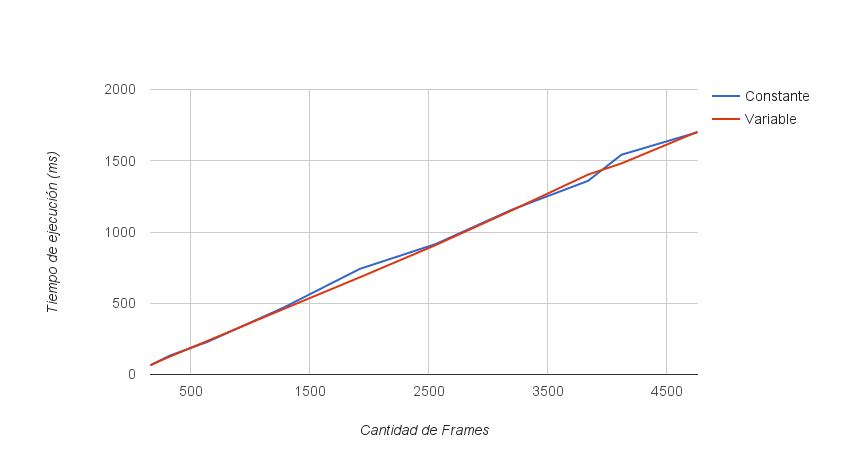
\includegraphics[width=0.70\columnwidth]{imagenes/tiempos/graf1_0.png}}
		\subfigure [M\'etodo Lineal] {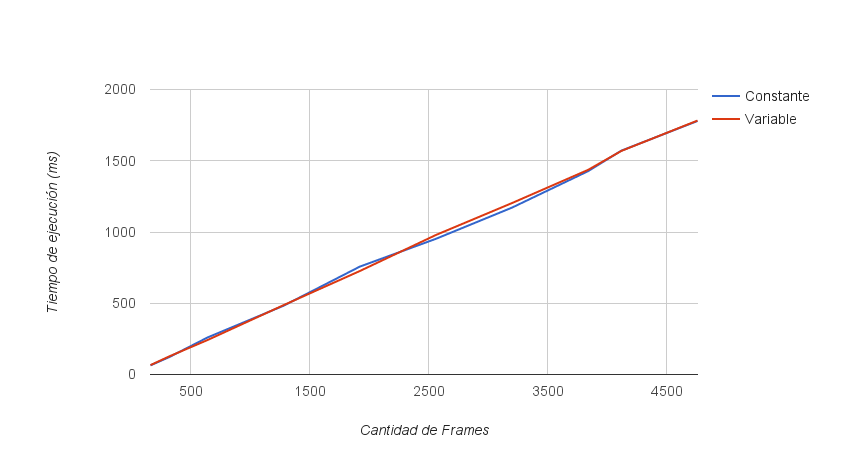
\includegraphics[width=0.49\columnwidth]{imagenes/tiempos/graf1_1.png}}
		\subfigure [M\'etodo de Splines naturales por bloques] {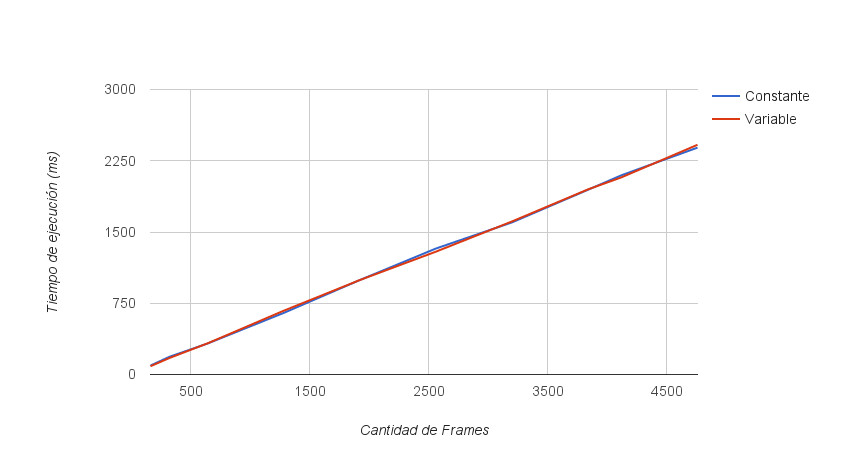
\includegraphics[width=0.49\columnwidth]{imagenes/tiempos/graf1_2.png}}
	\end{center}
\end{figure}


\par Como podemos observar en los gr\'aficos, los m\'etodos se comportan de la misma forma con ambas im\'agenes. Se notan diferencias en algunos momentos del m\'etodo del vecino mas cercano, pero manteniendo el mismo orden. No nos van a preocupar mucho estas diferencias, pero si las tendremos en cuenta de aqu\'i en adelante.
\par Luego de este experimento podemos asumir que el cambio de colores pr\'acticamente no va a influir en los tiempos de ejecuci\'on. Ahora s\'i podemos continuar con la experimentaci\'on teniendo en claro que ocurre con los colores.


\subsubsection{Experimento 2: Tiempos de ejecucí\'on vs Cantidad de Frames}
\par En este experimento vamos a comparar el tiempo de ejecuci\'on de los diferentes m\'etodos al aumentar la cantidad de frames de un video y tratar de determinar el orden de los mismos.

\par Para llevar a cabo el experimento vamos a crear videos con patrones de im\'agenes repetidos (tomando en consideraci\'on esos pequeños cambios que vimos en el experimento anterior) manteniendo el mismo ancho y alto de im\'agenes y cantidad de frames en aumento. La idea es fijar las variables de ancho (10px), alto (10px), variacion de colores (con un generador de patrones repetidos), frames intermedios (2) y tama~no de bloques (5)(para el caso del m\'etodo de Splines) para que no nos influyan en las mediciones y poder enfocarnos en la canidad de frames.

\subsubsubsection{Resultados del experimento 2}
\begin{figure}[ht]
	\begin{center}
		\subfigure [Tiempos de ejecuci\'on variando la cantidad de frames] {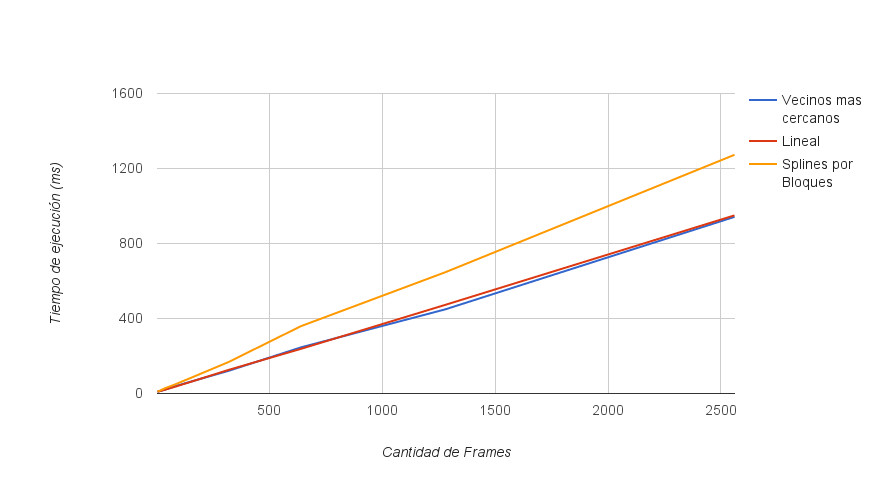
\includegraphics[width=0.9\columnwidth]{imagenes/tiempos/graf2.png}}
	\end{center}
\end{figure}
\par Luego de realizar el experimento podemos creer que el tiempo de ejecuci\'on de los tres m\'etodos es de orden lineal. Podemos notar que los Splines por Bloques se mantiene siempre por encima de los otros, pero mantienen su forma lineal. Mas adelante veremos las diferencias de calidad entre los m\'etodos y tendremos que tener en cuenta esta igualdad de orden, ya que no es tan grande como esper\'abamos en un principio. 

\paragraph{Cambios de inputs de entrada:}
De aquí en adelante realizaremos experimentos sobre 6 videos reales, con distintas calidades y duraciones. Los videos elegidos como inputs se encuentran en slow motion originalmente, y muestran situaciones que consideramos interesantes para analizar resultados cuantitativos y cualitativos, como por ejemplo, una pelota de tenis volando o fideos cayendo lentamente, ya que se pueden apreciar las diferencias con los videos originales más claramente.
\par A continuación una breve descripción de los videos de entrada que utilizamos para los tests: (de menor a mayor calidad)
\begin{multicols}{2}
\begin{itemize}
\item \textit{cupcake} : $\#$frames = 252, tamaño 240x360
\item \textit{perro} : $\#$frames = 252, tamaño 360x360
\item \textit{morocho} : $\#$frames = 452, tamaño 360x360
\item \textit{tenis} : $\#$frames = 450, tamaño 240x426
\item \textit{bebes} : $\#$frames = 225, tamaño 544x1280
\item \textit{fideos} : $\#$frames = 125, tamaño 720x1280
\end{itemize}
\end{multicols}


\subsubsection{Experimento 3: Tiempos de ejecucí\'on vs Tama\~no de Bloques}
\par Como tomamos la determinación de aplicar el m\'etodo de Splines de a bloques de frames, queremos medir cu\'anto nos afecta el tama\~no que decidamos darle a estos bloques en el tiempo de ejecuci\'on del m\'etodo.

\par Para esto vamos a tomar los videos antes mencionados, y correremos el m\'etodo de splines con diferentes tama\~nos de bloque. Mantendremos la cantidad de frames intermedios fija (2) Con esto observaremos el comportamiento del m\'etodo y podremos determinar cu\'anto nos afectar\'a el tama\~no de bloques en el rendimiento.

\subsubsubsection{Resultados del experimento 3}
\begin{figure}[ht]
	\begin{center}
		\subfigure [Tiempos de ejecuci\'on variando el tamaño de los bloques] {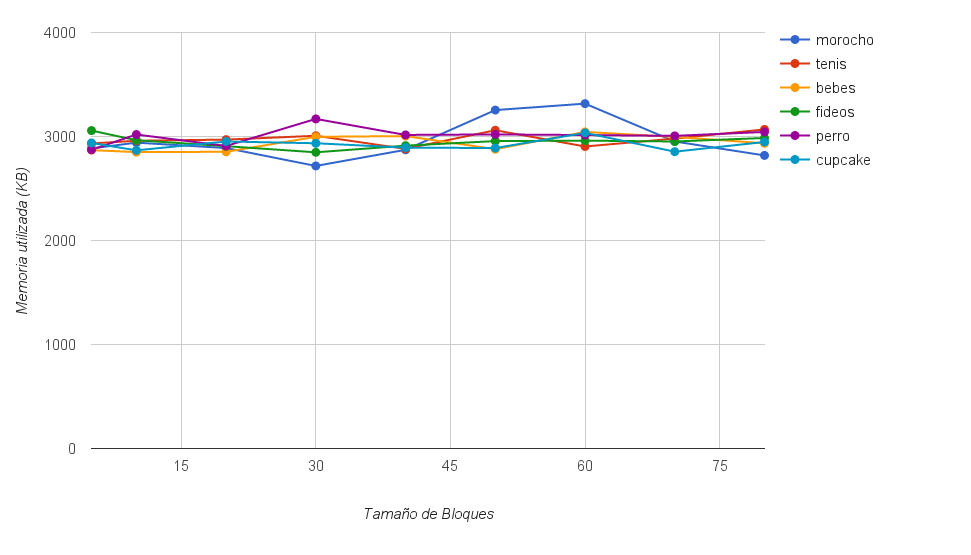
\includegraphics[width=1\columnwidth]{imagenes/tiempos/exp3_gabriel.png}}
	\end{center}
\end{figure}
\par Podemos observar que a pesar de algunas diferencias el orden del tiempo se mantiene constante y no se vi\'o afectado por el aumento del tama\~no de bloques. Nos parece normal que esto ocurra, ya que el algoritmo realiza la misma cantidad de pasos. La diferencia se ve en como se agrupan los datos, lo que si puede influir en las im\'agenes decididas a agregar como nuevos frames.



\subsubsection{Experimento 4: Tiempos de ejecucí\'on vs Cantidad de frames intermedios}
\par Vamos a observar como se comportan los m\'etodos al variar la cantidad de frames que se desean agregar. A pesar de que no se hacen muchos pasos extra para agregar un frame intermedio y solo se realiza una ecuaci\'on, esta ecuaci\'on se repite para cada pixel del nuevo frame. Creemos que esto va a afectar mucho en el tiempo de ejecuci\'on de los tres m\'etodos.
\par Correremos los distintos m\'etodos sobre los 6 videos antes mencionados aumentando la cantidad de frames intermedios y observaremos como se comportan seg\'un sus diferentes caracter\'isticas.

\subsubsubsection{Resultados del experimento 4}
\begin{figure}[ht]
	\begin{center}
		\subfigure [M\'etodo del Vecino mas Cercano] {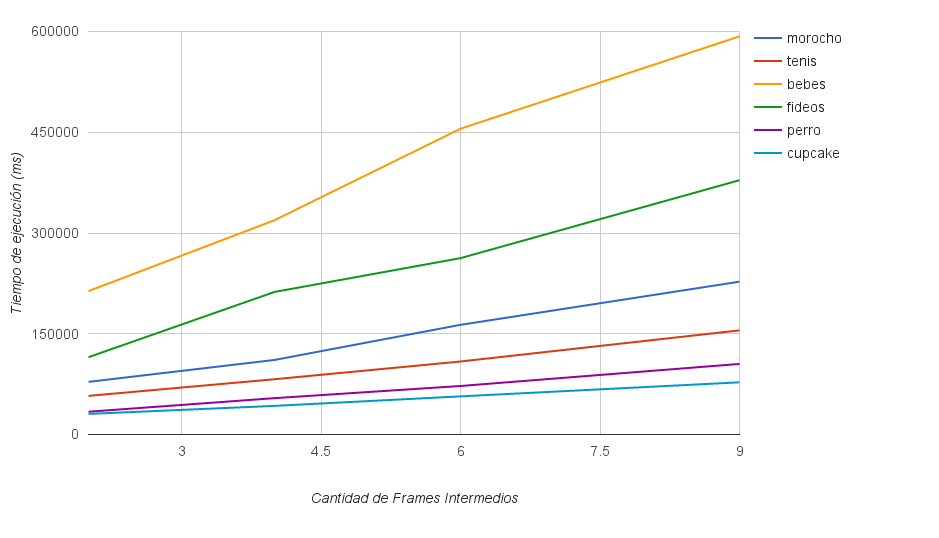
\includegraphics[width=0.9\columnwidth]{imagenes/tiempos/exp4_cercano.png}}
		\subfigure [M\'etodo Lineal] {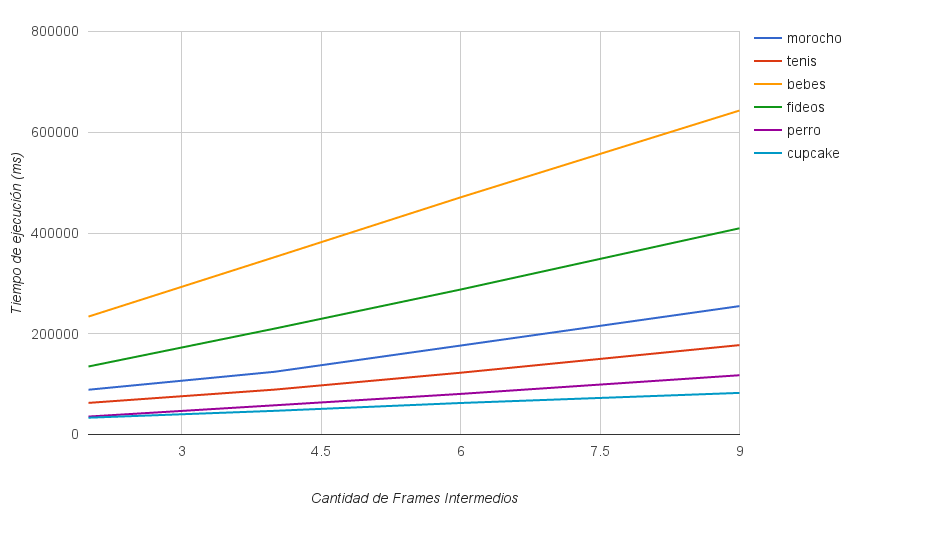
\includegraphics[width=0.49\columnwidth]{imagenes/tiempos/exp4_lineal.png}}
		\subfigure [M\'etodo de Splines Por Bloques] {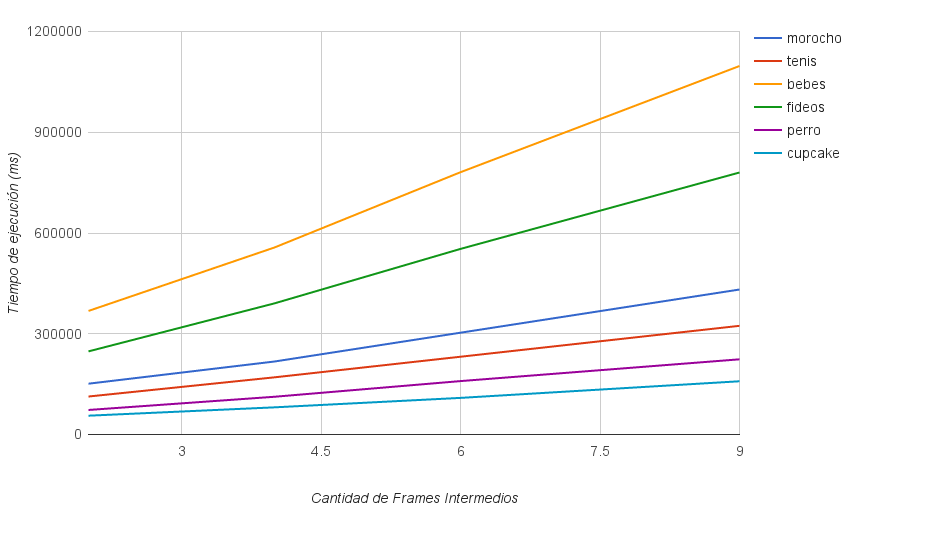
\includegraphics[width=0.49\columnwidth]{imagenes/tiempos/exp4_splines.png}}
	\end{center}
\end{figure}

\par Al ver los resultados lo primero que notamos en un \'orden similar y lineal entre los videos Cupcake, Tenis, Perro, Morocho. Los videos Bebes y Fideos mantienen ordenes mayores. Esto se lo adjudicamos al hecho de que son los videos con mayor resoluci\'on, y se ven mas afectados al agregar frames. Igualmente mantienen un orden lineal dentro de lo esperado.

\par Veamos mas en detalle el efecto de agregar un frame. Supangamos que tomamos N como la cantidad de frames del video original y F como cantidad de frames intermedios a agregar. De esta forma al aplicar alguno de los m\'etodos se agregan F frames N-1 veces $\longrightarrow$ F*(N-1). Si aplicamos uno de los m\'etodo nuevamente, pero esta vez con F+1 frames intermedios, se agregar\'an F+1 frames N-1 veces $\longrightarrow$ (F+1)*(N-1) = F*(N-1) + (N-1). Con este razonamiento simple y sin entrar en detalles podemos convencernos de que al aumentar la cantidad de frames aumentamos de forma lineal la cantidad de operaciones a realizar (agregamos N-1 operaciones `agregar frame intermedio').

\newpage

\subsection{Análisis Cuantitativo}
\par Para realizar un an\'alisis cuantitativo, llamamos $F$ al frame del video real (ideal) que deber\'iamos obtener con nuestro algoritmo, y sea $\bar{F}$ al frame del video efectivamente construido. Consideramos entonces dos medidas, directamente relacionadas entre ellas, como el \emph{Error Cuadr\'atico Medio} (ECM) y \emph{Peak to Signal Noise Ratio} (PSNR), denotados por $\texttt{ECM}(F,\bar{F})$ y $\texttt{PSNR}(F,\bar{F})$, respectivamente, y definidos como:
\begin{equation*}
\texttt{ECM}(F,\bar{F}) = \frac{1}{mn}\sum_{i=1}^m\sum_{j = 1}^n |F_{k_{ij}} - \bar{F}_{k_{ij}}|^2 \label{eq:ecm}
\end{equation*}
\noindent y
\begin{equation*}
\texttt{PSNR}(F,\bar{F}) = 10 \log_{10}\bigg(\frac{255^2}{\texttt{ECM}(F,\bar{F})}\bigg). \label{eq:psnr}
\end{equation*}
\par Ambas métricas se utilizan para medir la diferencia absoluta entre dos señales, en este caso entre los valores de los pixels del video de entrada y del de salida. Los algoritmos implementados para calcular ECM y PSNR calculan dichos valores frame a frame y luego hacen un promedio entre todos los frames del video. Utilizaremos estos promedios obtenidos para comparar la efectividad (en términos cuantitativos) de cada algoritmo, dependiendo de los parámetros de entrada. (El algoritmo para ECM puede encontrarse en el Apéndice \ref{ecmalgo}). 
\par Notar que en los casos en que el ECM entre dos frames sea 0, (debido a que dicho frame no se modificó), el PSNR da infinito. Para calcular el promedio del PSNR de un video, en estos casos, no se tomarán en cuenta dichos frames.

\subsubsection{Experimentación con ECM y PSNR}

\par Para calcular el ECM obtenido a partir de los videos generados con los algoritmos propuestos, implementamos tests que comparan frame a frame el video original ya en slow motion, con el video obtenido luego de eliminar frames intermedios y aplicar cada método para regenerar dichos frames. Es decir, si al video original le eliminamos 2 frames intermedios (utilizando la función \texttt{eliminarFrames}, ver Apéndice \ref{eliminarframes}), compararemos el video original con el video obtenido luego de aplicar cada uno de los algoritmos, tomando como parámetro la misma cantidad de frames intermedios que le habíamos eliminado al video en un principio, en este caso 2.
\par Realizaremos esto para 6 videos diferentes, con distintas calidades y duraciones. Los videos elegidos como inputs se encuentran en slow motion originalmente, y muestran situaciones que consideramos interesantes para analizar resultados cuantitativos y cualitativos, como por ejemplo, una pelota de tenis volando o fideos cayendo lentamente, ya que se pueden apreciar las diferencias con los videos originales más claramente. Además, analizaremos los resultados según el tamaño y calidad del video, ya que algunos algoritmos podrían mejorar su rendimiento en dichos casos. Creemos que videos de mayor calidad generan resultados de mayor precisión.
\par Los tests que generamos calculan el ECM para dichos inputs variando la cantidad de framesIntermedios eliminados al original (2, 4 o 6 frames) para cada algoritmo. Para el algoritmo de splines, a su vez, realiza el mismo cálculo tomando distintos tamaños de bloque (4, 8 o 16 frames por bloque). Con esto pretendemos observar cómo afectan estos parámetros cuantitativamente al resultado final. Bloques de splines de menor tamaño supondrían una mayor precisión debido a que los videos cambian de tomas rápidamente, y al prolongar el tamaño del bloque permite interpolar frames tomando como parámetros frames pertenecientes a distintas tomas, y por lo tanto generar resultados no deseados como imágenes transparentes entre una toma y otra. Estos \textit{artifacts} serán analizados con más detalle en la próxima sección de análisis cualitativo. Aquí nos limitaremos a analizar los resultados cuantitativos.
\par A continuación una breve descripción de los videos de entrada que utilizamos para los tests: (de menor a mayor calidad)
\begin{itemize}
\item \textit{cupcake} : $\#$frames = 252, tamaño 240x360
\item \textit{perro} : $\#$frames = 252, tamaño 360x360
\item \textit{morocho} : $\#$frames = 452, tamaño 360x360
\item \textit{tenis} : $\#$frames = 450, tamaño 240x426
\item \textit{bebes} : $\#$frames = 225, tamaño 544x1280
\item \textit{fideos} : $\#$frames = 125, tamaño 720x1280
\end{itemize}

\par  \textbf{En el Apéndice \ref{cuant} se puede encontrar una tabla con todos los valores obtenidos sobre el ECM promedio y los ECM máximos obtenidos por cada algoritmo para cada input. A continuación estudiaremos el comportamiento de cada método desde distintos enfoques.}

\subsubsection{Resultados sobre ECM y PSNR}

\subsubsubsection{Experimento 1: Efectividad de los métodos según ECM}

\par Comparamos la efectividad de los métodos según el ECM promedio obtenido en cada uno de los inputs con 2 frames intermedios eliminados. Cuanto menor sea el error, consideraremos que el método es más efectivo cuantitativamente. Dejaremos afuera el input \textit{perro} para que el gráfico de barras sea más claro, ya que son valores muy altos comparados a los demás.

\begin{figure}[ht]
	\begin{center}
		\subfigure [Efectividad de los métodos según ECM] {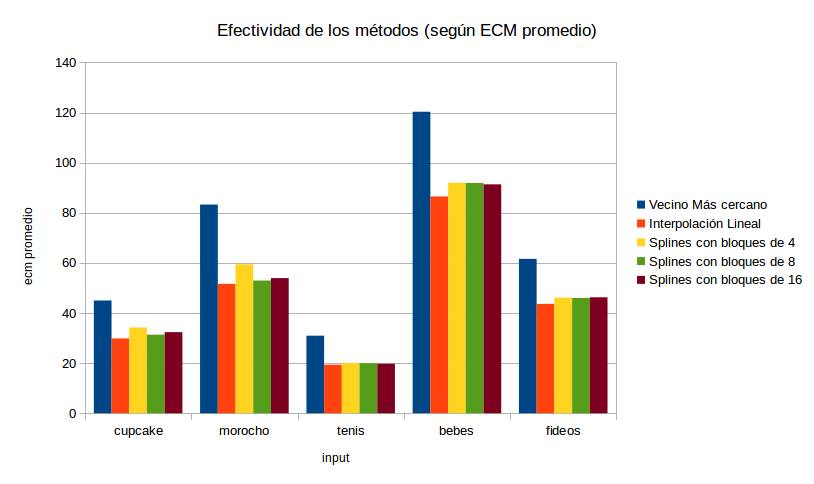
\includegraphics[width=0.9\columnwidth]{imagenes/cuantitativos/exp1.jpg}}
	\end{center}
\end{figure}

\par Se puede observar en el gráfico que el método que arroja mejores resultados con respecto al error cuadrático medio es el de Interpolación Lineal, a diferencia de lo que creíamos. Supusimos que splines por el mayor grado de complejidad de los cálculos y del polinomio interpolante daría como resultado videos más aproximados al original (ideal). Sucede que el algoritmo de splines divide los frames en bloques de como mínimo 4 frames para poder calcular el polinomio de grado 3 (4 variables), lo que hace que en varios de esos bloques los frames pertenezcan a tomas diferentes del video. Si los frames son de tomas diferentes, o los frames varían demasiado entre uno y otro, la función interpolante resultante tiene más error. Como el método lineal "divide" los frames en bloques de a 2, ya que realiza una función cada 2 frames, el impacto de este fenómeno es menor.
\par Además, se puede observar en el gráfico el impacto del \textbf{tamaño de bloque }tomado para realizar los splines. Variar el tamaño del bloque no modifica significativamente el error cometido, sin embargo, estimamos que al aumentar considerablemente el tamaño de los bloques se podrán observar errores visuales (más sobre esto en la sección Análisis Cualitativo).
\par Se puede observar que el tamaño de los videos y la calidad no impacta significativamente en el error cuadrático medio. Sin embargo, el video \textit{perro}  tiene mayores valores de error en todos los algoritmos (ver Apéndice), debido a que es el único de los videos que fue grabado con un celular en movimiento.
\par Por último, variar la calidad del video no trae grandes diferencias en términos cuantitativos, sin embargo, al observar los outputs, se nota una leve mejora del método de splines en términos cualitativos (se producen menos exploits). 

\subsubsubsection{Experimento 2: Impacto del parámetro Frames Internos eliminados}

\par Usando los mismos inputs, correremos los métodos tomando distintas cantidades de frames internos eliminados y compararemos los resultados. Aumentar la cantidad de frames internos a regenerar, debería aumentar el error cuadrático medio.

\begin{figure}[ht]
	\begin{center}
		\subfigure [Efectividad de los métodos según frames intermedios eliminados] {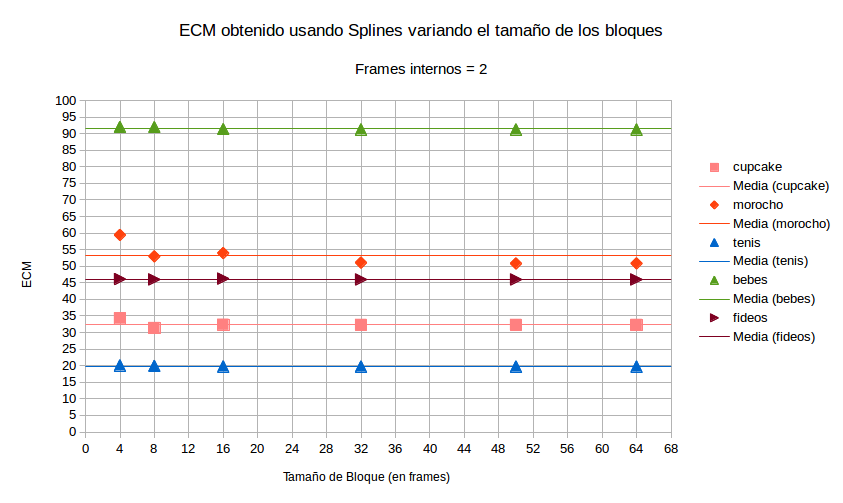
\includegraphics[width=0.9\columnwidth]{imagenes/cuantitativos/exp2.png}}
	\end{center}
\end{figure}

\par En el gráfico se muestran los valores obtenidos al calcular el promedio de los ECM de cada input generados por cada método, según cuál fue la cantidad de frames internos pasada por parámetro.
\par Efectivamente, aumentar framesIntermedios aumenta el error cuadrático medio. Se puede ver en el gráfico que lo hace linealmente, en todos los métodos. Esto se debe a que es mayor la cantidad de frames que se obtienen usando las funciones interpolantes, aumentando el error producido.

\subsubsubsection{Experimento 3: Efectividad de los métodos según PSNR}

\par El PSNR es la métrica utilizada con mayor frecuencia como medida de la calidad objetiva de video. Sin embargo, a causa del comportamiento nolineal del sistema visual humano los valores de PSNR no poseen una perfecta correlación con la calidad visual percibida. 
\par Análogamente, calculamos los PSNR promedio obtenidos con cada algoritmo para los mismos inputs mencionados anteriormente:

\begin{figure}[ht]
	\begin{center}
		\subfigure [Efectividad de los métodos según PSNR] {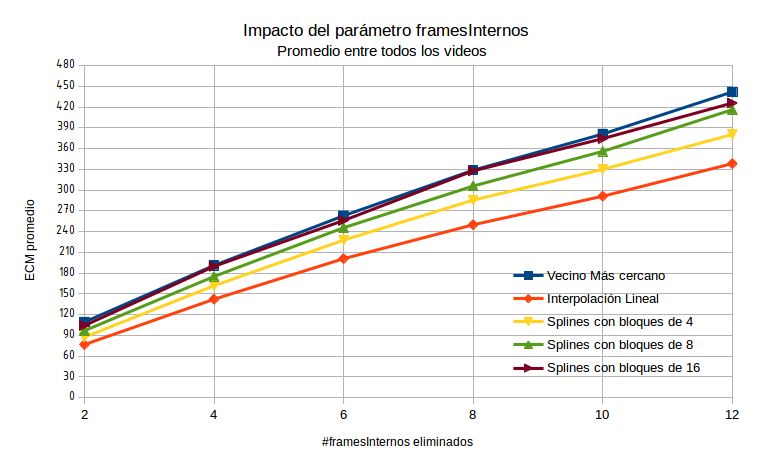
\includegraphics[width=0.9\columnwidth]{imagenes/cuantitativos/exp3.png}}
	\end{center}
\end{figure}

\bigskip

\newpage

\par Como era de esperar, los resultados se corresponden con los obtenidos a partir de comparar los ECM producidos por cada algoritmo. Por definición de PSNR, cuanto menor sea el error, mayor será el PSNR y por lo tanto mejor la calidad.
\par  Interpolación lineal es el método con mayor efectividad en términos cuantitativos.

%\subsubsection{Experimento 4: Usando números fraccionarios vs. enteros para calcular los frames Intermedios}
%
%\par Al momento de implementar el algoritmo de interpolación por splines, nos planteamos dos posibilidades para tomar los valores de los $[x_i]$ (frames del algoritmo). Se podría tener en cuenta los frames Intermedios que necesitamos regenerar o no. Es decir, por ejemplo, teniendo un video de 2 frames, y sabiendo que vamos a agregar 1 frame intermedio (es un caso hipotético, ya que con splines el mínimo es 4 frames), podríamos tener $x_0$ = 0, $x_1$ = 1 y calcular el frame intermedio tomando $x=\frac{1}{2}$ en la función interpolante; o tomar $x_0$ = 0, $x_1$ = 2 y usar $x=1$ para el frame intermedio. En otras palabras, podríamos tomar $h=1$ o $h=framesIntermedios+1$. ($h = x_{i+1} - x_i$)
%\par Este experimento tiene el objetivo de comparar los errores cuadráticos medios producidos por los 3 métodos, implementando ambas opciones, para comprobar nuestra hipótesis sobre que el error se reduce usando números enteros para los frames Intermedios.
%\par El siguiente gráfico muestra los resultados obtenidos al calcular el promedio de los ECM obtenidos para los mismos 6 inputs mencionados anteriormente:
%
%...




\newpage
\subsection{Análisis Cualitativo}
\par En esta secci\'on realizaremos un an\'alisis cualitativo de los m\'etodos desarrollados.
Con este fin, observaremos el resultado de aplicar los distintos m\'etodos a ciertas entradas; 
buscaremos \textit{artifacts} (errores visibles en el video causados por la interpolaci\'on), compararemos los diferentes procedimientos entre s\'i, y los efectos de distintos par\'ametros en cada uno.

\subsubsection{Artifacts}
\par Si bien encontrar una interpolaci\'on ideal puede no ser posible, se pueden generar frames intermedios que no sean completamentamente fidedignos a los id\'oneos, pero que son de todas formas veros\'imiles.
Un objetivo quiz\'as m\'as plausible que una interpolaci\'on perfecta o ideal, es una de la cual el observador no puede discernir de los frames originales (al menos en una observaci\'on ``normal''). 
Los \textit{artifacts} son errores en la interpolaci\'on que tienen un efecto visible en el video, y que detraen de este objetivo. 
Los estudiaremos con especial atenci\'on ya que tienen un significativo efecto negativo en la percibida calidad del video resultante.

\subsubsubsection{Vecino m\'as cercano}
\par La mayor\'ia de los m\'etodos de interpolaci\'on intentan ``adivinar'' los frames intermedios en base a los de referencia, lo que conlleva posibles errores.
Vecino m\'as cercano, por otro lado, genera a los intermedios copiando a los de referencia, por lo que no se pueden producir artifacts.

\subsubsubsection{Lineal y Splines}
\par Ambos m\'etodos funcionan de forma similar: viendo c\'omo var\'ian los valores de los mismo p\'ixeles (es decir, de los p\'ixeles que est\'an en la misma posici\'on de cada frame) entre los frames de referencia, e interpolando los valores de los intermedios.
Lo que var\'ia es la familia de funciones mediante la cual aproximan, y cu\'antos frames de referencia utilizan.
Debido a esto, ambos m\'etodos generan ``trazas'' al interpolar movimiento.
A continuaci\'on ahondaremos en esto, y daremos ejemplos.

\subsubsubsection{Lineal}
\par Si el video representa el movimiento (algo casi ubicuo en este tipo de aplicaciones) de alg\'un cuerpo a lo largo de los frames, lo que este m\'etodo hace es esencialmente un ``fade-in'' y ``fade-out'' del objeto del primer frame de referencia al segundo.
Para clarificar lo anterior: se observa que el objeto en el primer frame se va transformando en el fondo (en la posici\'on de dicho objeto) del segundo, mientras que el fondo (en la nueva posici\'on del objeto) del primero se va transformando en el objeto del segundo.
\par En la realidad (a escala no-cu\'antica), el movimiento es continuo, por lo que idealmente la interpolaci\'on deber\'ia generar frames intermedios donde el cuerpo en movimiento se encuentra en los puntos intermedios de dicho movimiento.
El m\'etodo lineal genera movimiento discontinuo, donde el cuerpo se funde de una posici\'on en un frame de referencia a la del pr\'oximo frame.
Un claro ejemplo de estas trazas o ``fade-in''-``fade-out'' se puede observar en la imagen \ref{TenisTrazaLineal}, que es un frame interpolado linealmente.

\FloatBarrier
\begin{figure}[h]
\caption{Traza en interpolacion lineal - video: Tenis con 6 frames intermedios}
\label{TenisTrazaLineal}
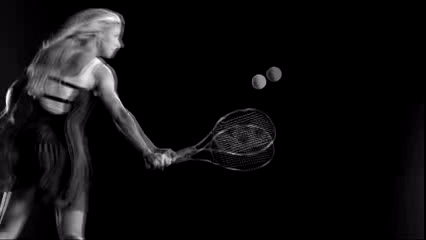
\includegraphics[width=0.9\columnwidth]{imagenes/cualitativos/TTL.png}
\end{figure}
\FloatBarrier

\par Si bien estas trazas t\'ecnicamente son artifacts, ya que no representan la realidad del video, cabe destacar que a los seres humanos \'estas no nos parecen muy fuera de lugar o inveros\'imiles; en dibujo, efectos especiales y dem\'as, una forma de representar movimiento es justamente mediante tales trazas; incluso nuestro propio sentido de visi\'on en ciertas circunstancias captura el movimiento de tal forma (como cualquiera habr\'a hecho en alg\'un momento, si uno mueve la mano r\'apidamente de un lado al otro con el brazo fijo se observan trazas en vez de un movimiento continuo - otro ejemplo es el cl\'asico truco del l\'apiz que parece hecho de goma). 
\par Debido a esto, las trazas pueden tener un impacto incluso positivo en el video en lo que concierne a interpolaci\'on del movimiento, en especial con framerate alto y pocos frames intermedios.

\subsubsubsection{Splines}
\par En el m\'etodo de Splines se observan trazas similares a las de la interpolaci\'on lineal; la diferencia yace en c\'omo se ve el ``fade-in''-``fade-out''.
Un ejemplo de tales trazas, para el mismo video que el de la imagen \ref{TenisTrazaLineal}, se encuentra en la figura \ref{TenisTrazaSplines}.

\FloatBarrier
\begin{figure}[h]
\caption{Traza en Splines - video: Tenis con 6 frames intermedios, tama\~no de bloque 4}
\label{TenisTrazaSplines}
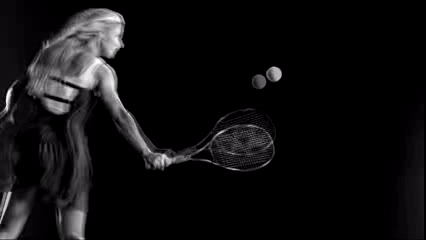
\includegraphics[width=0.9\columnwidth]{imagenes/cualitativos/TTS.png}
\end{figure}
\FloatBarrier

\par Cabe destacar que el m\'etodo de Splines emplea varios frames en la interpolaci\'on, a diferencia de Lineal, por lo que en ciertos casos la traza puede describir a un objeto no s\'olo en un frame y el siguiente, pero en m\'ultiples frames consecutivos.
Un tal caso se puede observar en la figura \ref{FideosSplinesTrazaArtifact}; en el video original, en la regi\'on del frame del cual extrajimos la imagen hay un s\'olo objeto cayendo, pero al interpolarlo se ven 4 trazas (dos con una tonalidad clara, dos con una oscura).
Si bien este efecto puede pasar desapercibido con un framerate alto, se vuelve m\'as notable al reducirlo, y tiene un impacto negativo en la interpolaci\'on desde un punto de vista cualitativo.

\FloatBarrier
\begin{figure}[h]
\caption{Traza en Splines - video: Fideos con 6 frames intermedios, tama\~no de bloque 50}
\label{FideosSplinesTrazaArtifact}
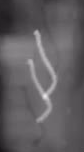
\includegraphics[width=0.9\columnwidth]{imagenes/cualitativos/FSTA.png}
\end{figure}
\FloatBarrier

\par Queremos comprender el efecto del tama\~no de bloques en la traza para Splines.
Con este fin, analizamos distintos videos; en esta secci\'on nos concentraremos en dos: uno de Tenis (del cual fueron sacadas las im\'agenes previamente utilizadas \ref{TenisTrazaLineal} y \ref{TenisTrazaSplines}), y uno de cupcakes.
Elegimos estos videos en particular ya que la pelota en el de Tenis es un objeto claro, isolado, contra un fondo negro, y por ende permite observar muy claramente la diferencia entre las trazas; 
utilizamos el de cupcakes ya que presenta un caso m\'as general que Tenis, ya que hay muchos objetos en movimiento de muchos colores distintos, y el fondo tambi\'en var\'ia.
Las siguientes im\'agenes son los frames intermedios entre dos posiciones consecutivas (en el video original) de la pelota en Tenis, para tama\~no de bloque 4 y 50, comparados lado a lado.

\FloatBarrier
\begin{figure}
\hfill
\subfigure[Tama\~no de bloque 4]{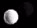
\includegraphics[width=.4\linewidth]{imagenes/cualitativos/Frames/S4F1.png}}
\hfill
\subfigure[Tama\~no de bloque 50]{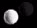
\includegraphics[width=.4\linewidth]{imagenes/cualitativos/Frames/S50F1.png}}
\hfill
\caption{Frame 1 - Tenis con 6 frames intermedios}
\end{figure}

\begin{figure}
\hfill
\subfigure[Tama\~no de bloque 4]{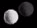
\includegraphics[width=.4\linewidth]{imagenes/cualitativos/Frames/S4F2.png}}
\hfill
\subfigure[Tama\~no de bloque 50]{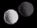
\includegraphics[width=.4\linewidth]{imagenes/cualitativos/Frames/S50F2.png}}
\hfill
\caption{Frame 2 - Tenis con 6 frames intermedios}
\end{figure}

\begin{figure}
\hfill
\subfigure[Tama\~no de bloque 4]{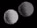
\includegraphics[width=.4\linewidth]{imagenes/cualitativos/Frames/S4F3.png}}
\hfill
\subfigure[Tama\~no de bloque 50]{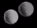
\includegraphics[width=.4\linewidth]{imagenes/cualitativos/Frames/S50F3.png}}
\hfill
\caption{Frame 3 - Tenis con 6 frames intermedios}
\end{figure}

\begin{figure}
\hfill
\subfigure[Tama\~no de bloque 4]{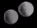
\includegraphics[width=.4\linewidth]{imagenes/cualitativos/Frames/S4F4.png}}
\hfill
\subfigure[Tama\~no de bloque 50]{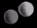
\includegraphics[width=.4\linewidth]{imagenes/cualitativos/Frames/S50F4.png}}
\hfill
\caption{Frame 4 - Tenis con 6 frames intermedios}
\end{figure}

\begin{figure}
\hfill
\subfigure[Tama\~no de bloque 4]{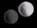
\includegraphics[width=.4\linewidth]{imagenes/cualitativos/Frames/S4F5.png}}
\hfill
\subfigure[Tama\~no de bloque 50]{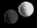
\includegraphics[width=.4\linewidth]{imagenes/cualitativos/Frames/S50F5.png}}
\hfill
\caption{Frame 5 - Tenis con 6 frames intermedios}
\end{figure}

\begin{figure}
\hfill
\subfigure[Tama\~no de bloque 4]{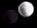
\includegraphics[width=.4\linewidth]{imagenes/cualitativos/Frames/S4F6.png}}
\hfill
\subfigure[Tama\~no de bloque 50]{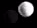
\includegraphics[width=.4\linewidth]{imagenes/cualitativos/Frames/S50F6.png}}
\hfill
\caption{Frame 6 - Tenis con 6 frames intermedios}
\end{figure}
\FloatBarrier

\par Se observa que la traza se describe con mayor intensidad (se ve m\'as claramente la pelota en su nueva posici\'on) al aumentar el tama\~no de bloques.
Esto hace que la interpolaci\'on del movimiento resulte m\'as gradual para bajo tama\~no de bloques, mientras que para una alta cantidad de bloques hay una diferencia m\'as marcada entre un frame original y el primer frame intermedio consecuente, lo que tiene un impacto cualitativo negativo en la interpolaci\'on.
\par Otro ejemplo de este efecto del tama\~no de bloques se puede ver en las siguientes im\'agenes, pertenecientes al video de cupcakes.
Nuevamente se puede observar que la traza para mayor cantidad de bloques se manifiesta con mayor intensidad, incluso al variar los colores de los objetos en movimiento y el color del fondo.

\FloatBarrier
\begin{figure}
\hfill
\subfigure[Tama\~no de bloque 4]{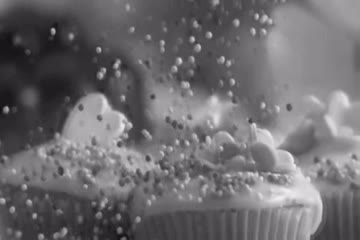
\includegraphics[width=.4\linewidth]{imagenes/cualitativos/Frames/CS4.png}}
\hfill
\subfigure[Tama\~no de bloque 50]{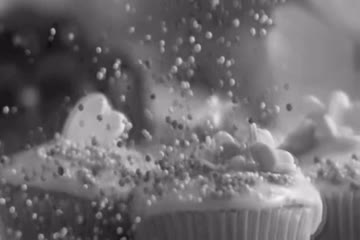
\includegraphics[width=.4\linewidth]{imagenes/cualitativos/Frames/CS50.png}}
\hfill
\caption{Cupcakes con 6 frames intermedios}
\end{figure}
\FloatBarrier

\subsubsection{Cambio de Escena}
\par Los componentes (en el sentido, de objetos, cuerpos, paisajes y dem\'as) de un video pueden pasar de un frame al otro esencialmente de tres maneras: 
se pueden quedar quietos (en cuyo caso los tres m\'etodos empleados las mantendr\'an iguales como deben, y por ende sin artifacts),
se pueden mover de alg\'un lugar del video al otro (los efectos de los m\'etodos de interpolaci\'on en el movimiento fueron detallados en la secci\'on previa),
o pueden aparecer/desaparecer (o saltar de un lugar a otro de una forma discontinua).
\par Cuando desaparece toda la escena y aparece una enteramente nueva, se dice que hubo un cambio de escena.
\'Este es el caso que analizaremos, ya que en las im\'agenes resultantes se ve con mayor claridad los efectos de los distintos m\'etodos de interpolaci\'on, pero todo lo que detallaremos en esta secci\'on se aplica perfectamente en el caso de que s\'olo algunos componentes aparezcan o desaparezcan.
\par El caso de cambio de escena es distinto que el de movimiento (real, el ficticio que no necesariamente es continuo lo contemplamos como aparici\'on/desaparici\'on por lo que se detallar\'a a continuaci\'on), ya que no necesariamente sabemos que es una transici\'on continua. 
Es perfectamente posible que la transici\'on de escenas sea un ``fade-out'' de una y un ``fade-in'' de otra, o que sea un corte limpio en el cual todo frame pertenece exclusivamente a una u otra (de hecho, ambas transiciones son usadas ampliamente en la cinematograf\'ia), o incluso mediante alguna otra t\'ecnica (como ejemplo, considerar las distintas formas de pasar de una diapositiva a otra en PowerPoint).
Adicionalmente, en ciertos casos es directamente imposible determinar cu\'al m\'etodo de transici\'on se utiliz\'o realmente (por ejemplo si el input es un subconjunto de frames de un cierto video original, y s\'olo se tienen frames anteriores y posteriores a la transici\'on).
\par Debido a esto, no consideraremos la forma en que los m\'etodos terminan efectuando el cambio de escena como errores o artifacts.
De todas modos, observaremos tales formas como parte de nuestro an\'alisis cualitativo.

\subsubsubsection{Vecino m\'as cercano}
\par Los frames intermedios a los de dos escenas distintas (es decir, los que representan tal cambio de escena) en este m\'etodo ser\'an copias del frame m\'as cercano, por lo que resultar\'an en una transici\'on ``limpia'', repentina, que pasa de una escena a la otra sin frames que pertenecen a ambas.

\subsubsubsection{Lineal y Splines}
\par El m\'etodo lineal resultar\'a en un ``fade-in''-``fade-out'' entre las escenas, con todos los frames intermedios pertenecientes a ambas.
Un ejemplo de esta transici\'on se puede ver en la imagen \ref{BebesLinealTransicion}, que corresponde a un frame intermedio a dos escenas distintas (en la escena saliente se ve al beb\'e con mayor zoom, en la entrante con menor).

\FloatBarrier
\begin{figure}[h]
\caption{Transicion Lineal - video: Bebes con 6 frames intermedios}
\label{BebesLinealTransicion}
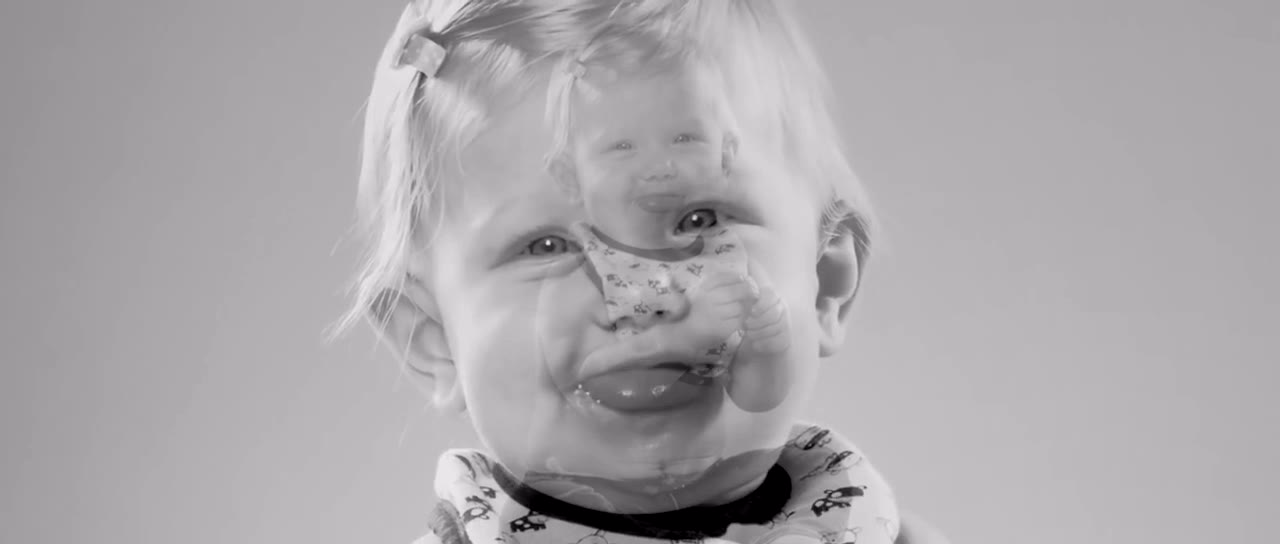
\includegraphics[width=0.9\columnwidth]{imagenes/cualitativos/BLT.png}
\end{figure}
\FloatBarrier

\par El uso de Splines resulta en el mismo tipo de transici\'on que la interpolaci\'on lineal (ejemplo: figura \ref{BebesSplinesTransicion}).
Nuevamente, la diferencia entre ambos yace en la intensidad de cada escena en el ``fade-in''-``fade-out''.

\FloatBarrier
\begin{figure}[h]
\caption{Transicion en Splines - video: Bebes con 6 frames intermedios, tama\~no de bloque 4}
\label{BebesSplinesTransicion}
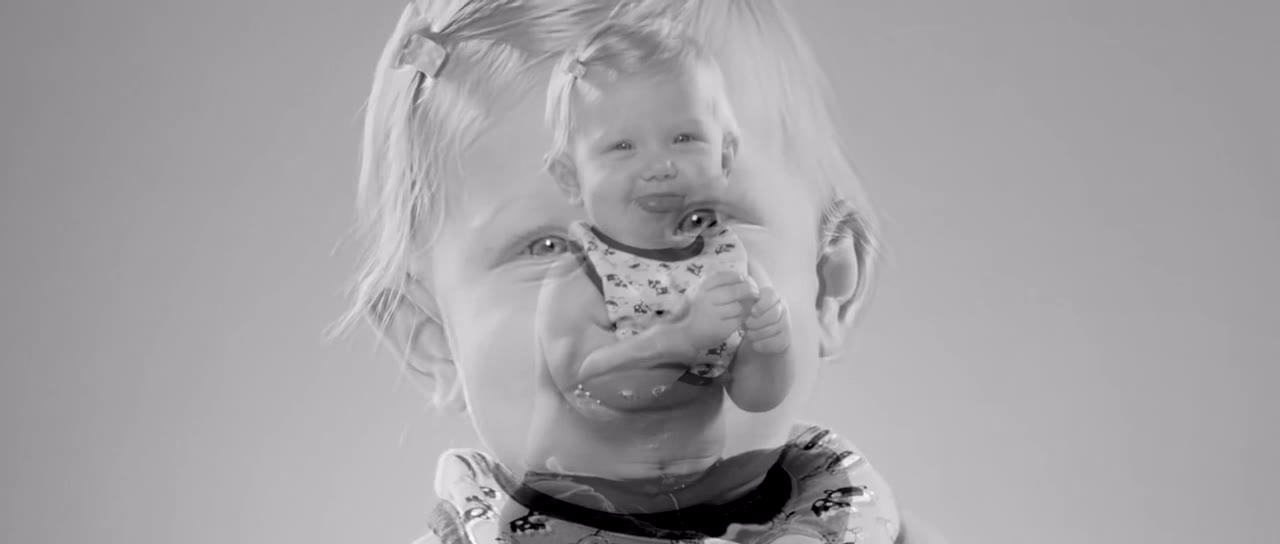
\includegraphics[width=0.9\columnwidth]{imagenes/cualitativos/BST.png}
\end{figure}
\FloatBarrier

\par Sin embargo, Splines utiliza varios frames de referencia, por lo que en algunos casos otra escena puede alterar frames que no son de transici\'on de una a otra.
Por ejemplo, consideremos 4 frames de un video: $f_1,\ f_2,\ f_3\ y\ f_4$.
Supongamos que $f_1$ y $f_2$ corresponden a una escena (llam\'emosla $S_1$), y que $f_3$ y $f_4$ corresponden a otra ($S_2$).
Los frames intermedios entre $f_2\ y f_3$ (denomin\'emoslos $f_{2-3}$) son los de transici\'on entre $S_1 y S_2$, y son los que llevar\'an a cabo el cambio de escena.
Sin embargo, los frames $f_{1-2}$ (utilizando la nomenclatura reci\'en detallada) pertenecen a una s\'ola escena ($S_1$), y por lo tanto esperamos que otras escenas ($S_2$, en este caso) no alteren los frames interpolados.
Si esto sucede, se producen artifacts donde pedazos de im\'agenes de otras escenas aparecen y desaparecen a pesar de que no tengan relaci\'on con el resto de la imagen.
Un ejemplo de esto se puede ver en la figura \ref{BebesSplinesArtifact}\footnote{En caso de que no se vea a primera vista el artifact, prestar particular atenci\'on a la frente y nariz del beb\'e, donde se puede observar una figura en negativo}.
Utilizando la notaci\'on previamente detallada, $S_1$ ser\'ia el beb\'e sentado (en la figura \ref{BebeSplinesS1} se ve un frame de esta escena), $S_2$ el zoom a la cara del beb\'e (en la figura \ref{BebeSplinesS2} se ve un frame de esta escena) y la imagen del artifact es uno de los frames $f_{3-4}$.
Al incrementar el tama\~no de bloque, incrementa la posibilidad de incurrir en este artifact, ya que se aumenta la cantidad de frames de una escena que son afectados por otra.

\FloatBarrier
\begin{figure}[h]
\caption{Artifact de transicion en Splines - video: Bebes con 6 frames intermedios, tama\~no de bloque 50}
\label{BebesSplinesArtifact}

\includegraphics[width=0.9\columnwidth]{imagenes/cualitativos/BSA.png}
\end{figure}
\FloatBarrier

%\FloatBarrier
%\begin{figure}[h]
%\caption{Escena 1 - video: Bebes con 6 frames intermedios, tama\~no de bloque 50}
%\label{BebesSplinesS1}
%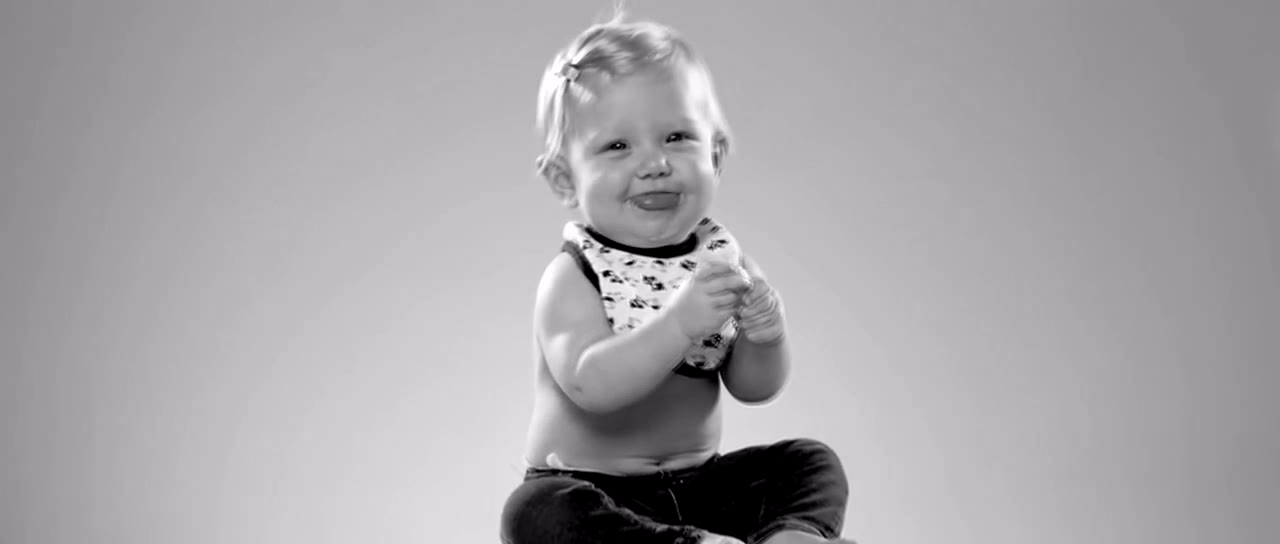
\includegraphics[width=0.9\columnwidth]{imagenes/cualitativos/BSS1.png}
%\end{figure}
%\FloatBarrier
%
%\FloatBarrier
%\begin{figure}[h]
%\caption{Escena 2 - video: Bebes con 6 frames intermedios, tama\~no de bloque 50}
%\label{BebesSplinesS2}
%
\includegraphics[width=0.9\columnwidth]{imagenes/cualitativos/BSS2.png}
%\end{figure}
%\FloatBarrier

\subsubsection{Comparaci\'on de la calidad de los m\'etodos}
\par En lo que concierne a Splines y Lineal contra Vecino m\'as cercano, observamos que el efecto de trazas presente en los primeros genera un efecto m\'as din\'amico y fluido en los videos, en contraposici\'on al efecto m\'as est\'atico de este \'ultimo.
Si bien la decisi\'on de cu\'al es mejor es subjetiva, personalmente nos pareci\'o que en videos de movimiento, Splines y Lineal eran mejores.
En videos que consisten mayoritariamente de cambios de escena (un slideshow de fotos, por ejemplo), depende de la opinion personal de cada uno con respecto al m\'etodo de transici\'on preferido.
\par En lo que concierne a Splines y Lineal, observamos que la traza es m\'as visible (se nota m\'as desde el punto de vista consciente), y nos pareci\'o que era preferible la traza m\'as sutil de interpolaci\'on lineal.
Esto, junto a los artifacts de transici\'on en Splines, nos llevan a recomendar la interpolaci\'on lineal por sobre este m\'etodo.


 
\newpage

\section{Conclusiones}

\par Desde el punto de vista cualitativo, no recomendamos utilizar Splines, debido a los \textit{artifacts} causados por \'este m\'etodo. Adicionalmente, recomendamos interpolaci\'on lineal sobre vecino m\'as cercano, en especial para mayor cantidad de frames intermedios.
 
\newpage

\section{Ap\'endices}

\subsection{Apéndice A}


 
\newpage

\section{Referencias}

\begin{thebibliography}{1}


%\bibitem{Brin1998}
%Sergey Brin and Lawrence Page.
%\newblock {The anatomy of a large-scale hypertextual Web search engine}.
%\newblock {\em Computer Networks and ISDN Systems}, 30(1-7):107--117, April
%  1998.

\end{thebibliography}


\end{document}
